\documentclass[12pt,a4paper]{report}

%----------------------------------------------------------------------------------------
%   PACKAGES
%----------------------------------------------------------------------------------------
\usepackage[francais]{babel} %French language package
\usepackage[utf8]{inputenc} %UTF8
\usepackage[T1]{fontenc} %For the acute french accents
\usepackage[pdftex]{graphicx} %To add figures in the document
\usepackage{hyperref} % To make hyperlinks in the document
\usepackage{amsthm} % To add mathematical symbols
\usepackage{pdfpages}

\usepackage{titlesec}
\titleformat{\chapter}[display]   
{\normalfont\huge\bfseries}{\chaptertitlename\ \thechapter}{20pt}{\Huge}   
\titlespacing*{\chapter}{0pt}{-50pt}{40pt}

\makeatletter
\setlength{\@fptop}{0pt}
\makeatother
\begin{document}
%----------------------------------------------------------------------------------------
%   TITLE PAGE
%----------------------------------------------------------------------------------------
\begin{titlepage}
\newcommand{\HRule}{\rule{\linewidth}{0.5mm}} % Defines a new command for the horizontal lines
\center

%----------------------------------------------------------------------------------------
%   LOGOS SECTION
%----------------------------------------------------------------------------------------

\includegraphics[scale=0.5]{images/umLogo.png} % Université de Montpellier Logo
\hspace{\fill}

\includegraphics[scale=0.25]{images/fdsLogo.jpg} % Faculté de Sciences Logo

%----------------------------------------------------------------------------------------
%   HEADING SECTIONS
%----------------------------------------------------------------------------------------
\textsc{\LARGE M1 Informatique AIGLE}\\[1cm]
\textsc{\Large \textbf{HMIN204}}\\[0.25cm]
\textsc{\large Conduite de Projet}\\[0.5cm]

%----------------------------------------------------------------------------------------
%   TITLE SECTION
%----------------------------------------------------------------------------------------
\HRule \\[0.4cm]
{ \huge \bfseries Méta-Rapport du TER}\\[0.4cm]
\HRule \\[0.5cm]

%----------------------------------------------------------------------------------------
%   AUTHORS AND SUPERVISORS SECTION
%----------------------------------------------------------------------------------------
{ \huge \bfseries Groupe \textsc{Bajonim}}\\[0.4cm]
\begin{minipage}{0.4\textwidth}
\centering \small
\textbf{Bachar \textsc{Rima}}, \\ \href{mailto:bachar.rima@etu.umontpellier.fr}{bachar.rima@etu.umontpellier.fr}\\ % Student
\textbf{Joseph \textsc{Saba}}, \\ \href{mailto:joseph.saba@etu.umontpellier.fr}{joseph.saba@etu.umontpellier.fr}\\ % Student
\textbf{Tasnim \textsc{Shaqura}}, \\ \href{mailto:tasnim.shaqura@etu.umontpellier.fr}{tasnim.shaqura@etu.umontpellier.fr}\\ % Student
\end{minipage} \\[0.8cm]

\begin{center}

\emph{Responsable de l'UE:} \\
Eric \textsc{Bourreau} % UE Supervisor
\end{center}

%----------------------------------------------------------------------------------------
%   DATE SECTION
%----------------------------------------------------------------------------------------
{\large 22 Mai 2019}\\[1cm]
\hspace{\fill}
\vfill % Fill the rest of the page with whitespace
\end{titlepage}

\tableofcontents
\chapter{Sujet}
Le logiciel constitue une partie trés importante de nos connaisances scientifiques, culturelles, et technique. Les logiciels sont présents dans tous les aspects de notre vie quotidienne. Il est donc important d'archiver les logiciels.\newline
Des efforts ont déja été fait pour la préservation des logiciels, tel que The Internet Archive et UNESCO Persist, mais ils se concentrent sur la préservation des éxécutables.
Software Heritage est un projet qui a comme but la préservation des codes source des logiciels disponibles publiquement. Les codes source sont importants parcequ'ils peuvent être façilement compris par des humains, et peuvent être façilement transformés en éxécutables.\newline
L'équipe de Software Heritage on crée une architecture qui permet de retrouver les sources codes d'un dépôt et de les placer dans l'archive. Les \textbf{Listers} sont une partie centrale à cette architecture. Ce sont des crawlers configurés pour parcourir des dépot de code et retrouver leurs contenu. Les differents dépôts de code ont des structures bien différentes l'un de l'autre, ce qui necessite la création d'un Lister dédié à chaque platforme qu'on souhaite archiver. L'équipe de Software Heritage a déja crée des Listers pour quelques dépots populaires, tel que Github et Bitbucket, avec succés; mais jusqu'à présent, aucune équipe externe a crée un Lister. Le dépôt que nous avons choisi est Launchpad.
\newline
Les objectifs de ce TER sont:
\begin{itemize}
  \item Lire et comprendre les articles publiés par l'équipe de Software Heritage
  \item Lire les tutoriels écrits par l'équipe de Software Heritage
  \item Tester differents dépot de code
  \item Écrire un Lister pour le dépot choisis
  \item Répliquer localement l'environnement de Software Heritage et tester le Lister
  \item Faire une Pull Request pour ajouter le Lister à Software Heritage
\end{itemize}
\chapter{Planning}
Dans ce chapitre, nous montrons le diagramme de Gantt initiale et le diagramme de Gantt final, puis nous analyserons les differences entre les deux. 
\section{Planning Prévisionel}
\begin{figure}[!ht]
\hspace*{-3.5cm}                
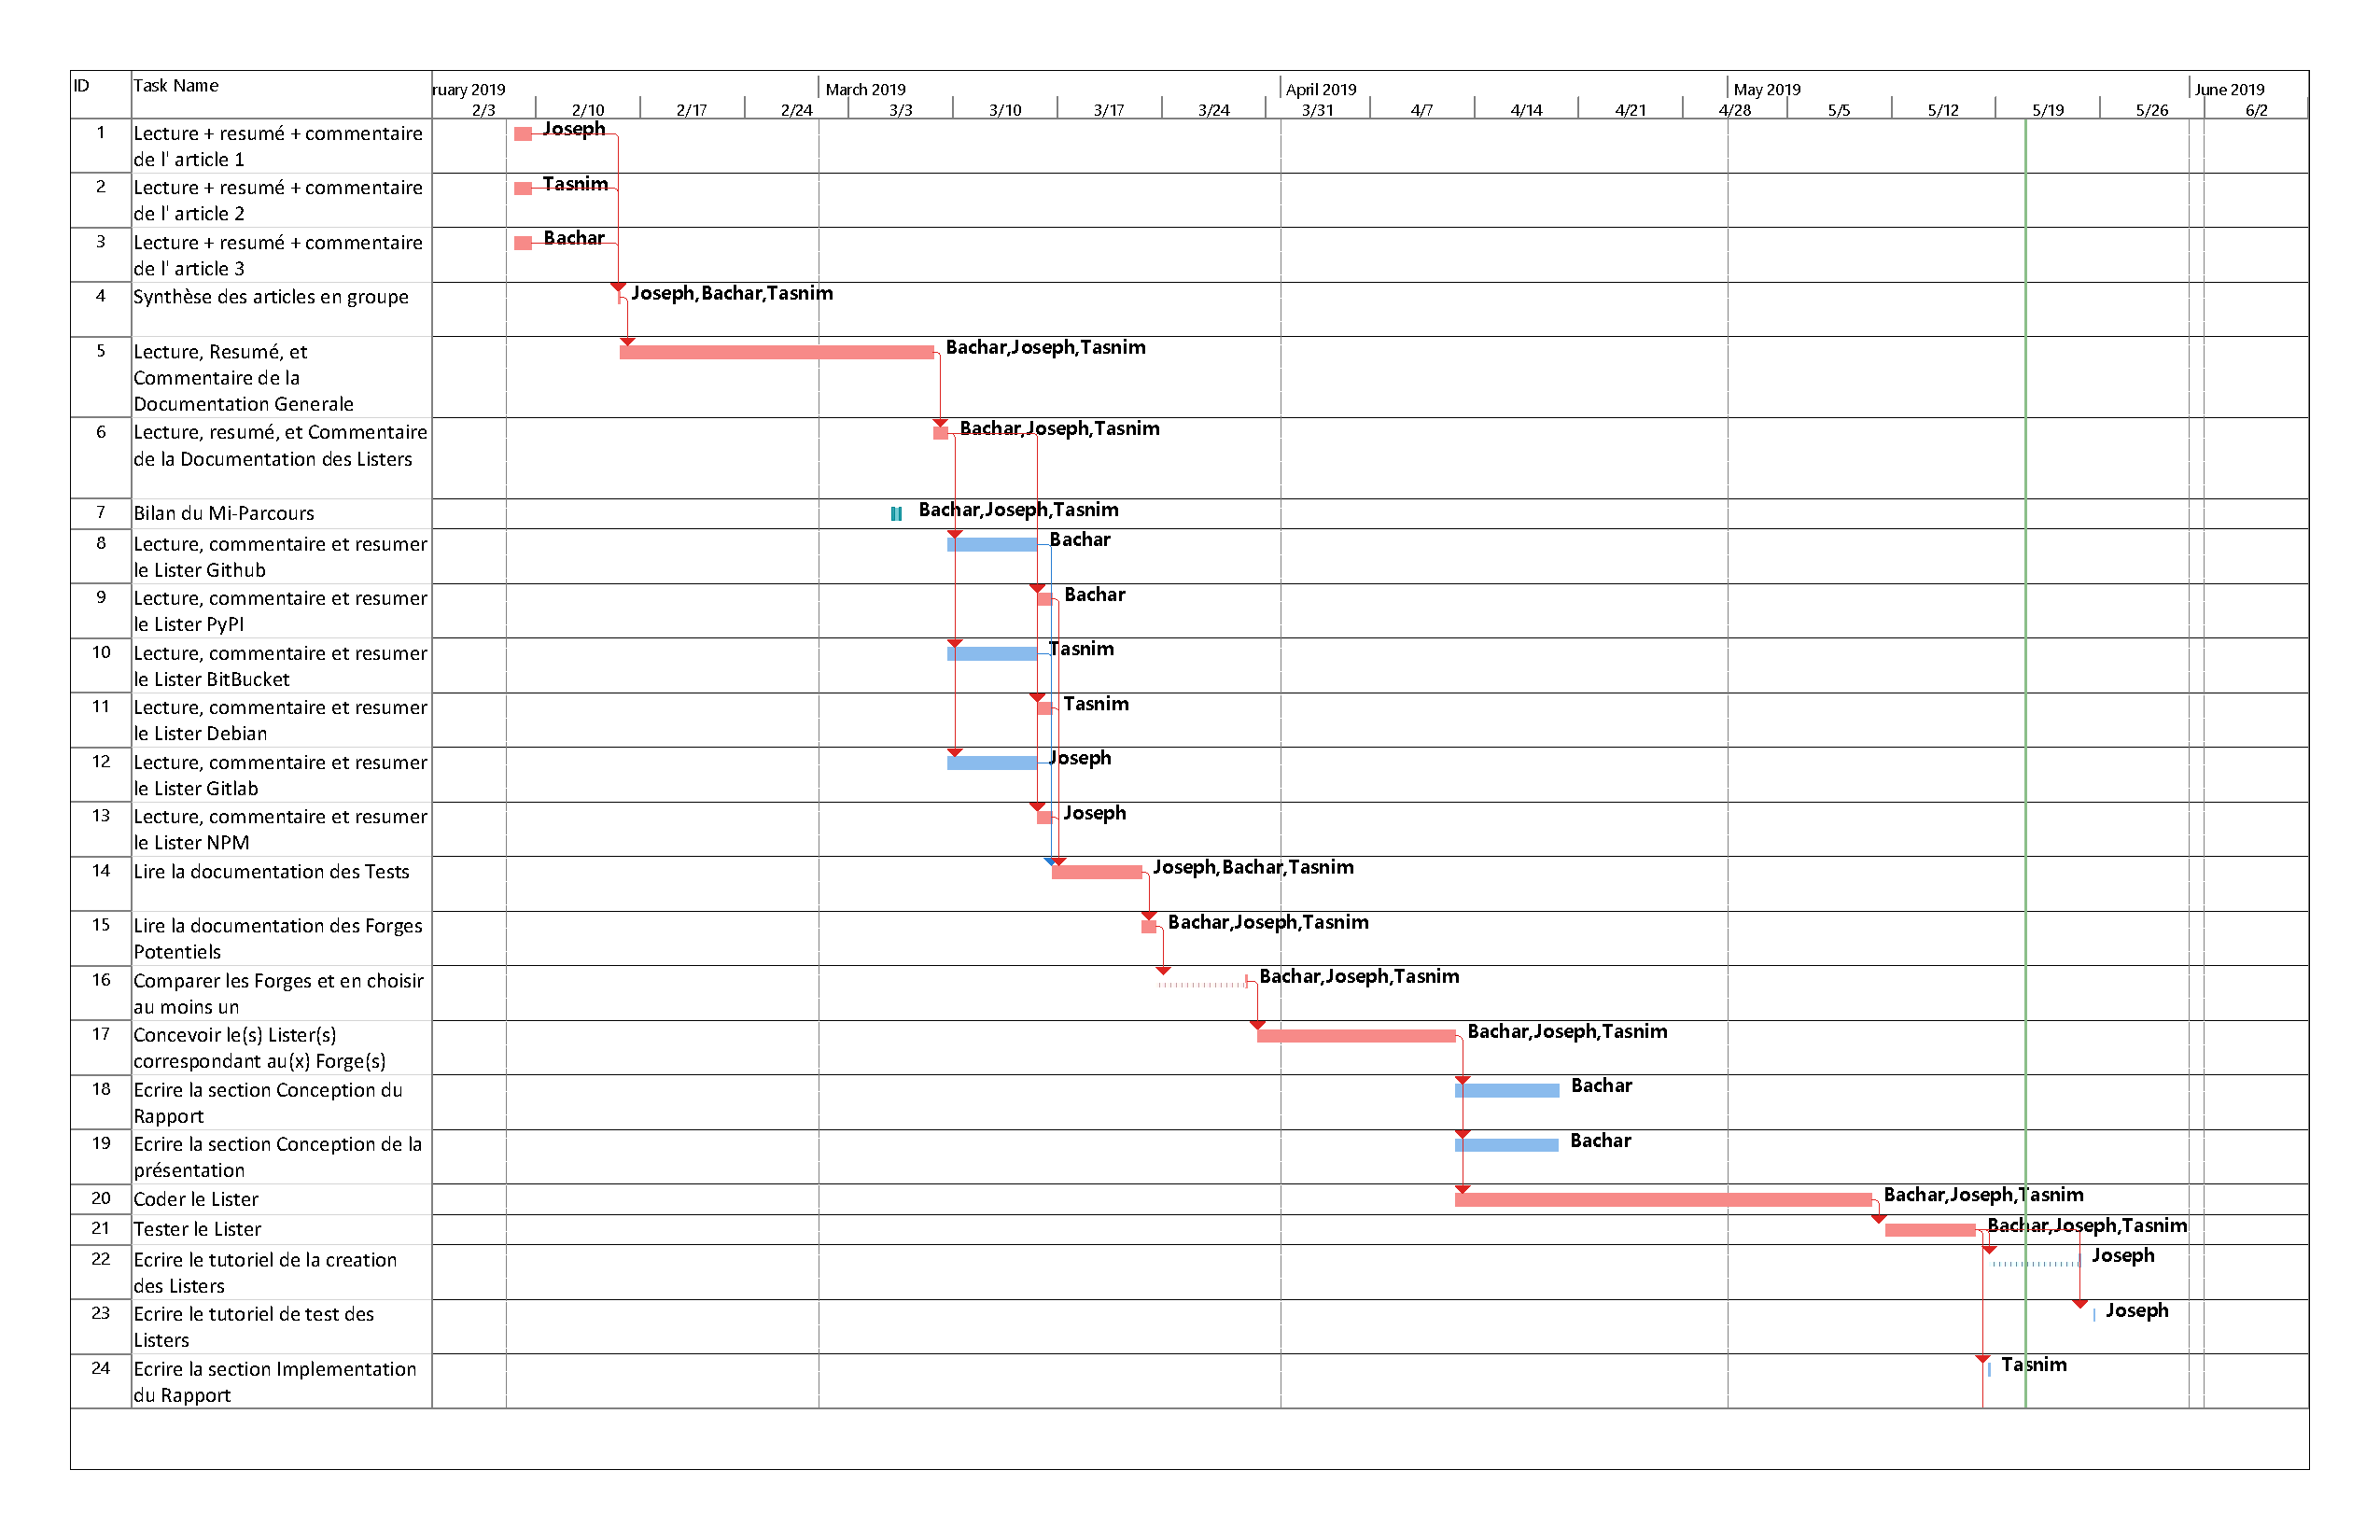
\includegraphics[scale=0.48]{feuille_de_route.pdf}
\end{figure}

\begin{figure}[!ht]
\hspace*{-3cm}                
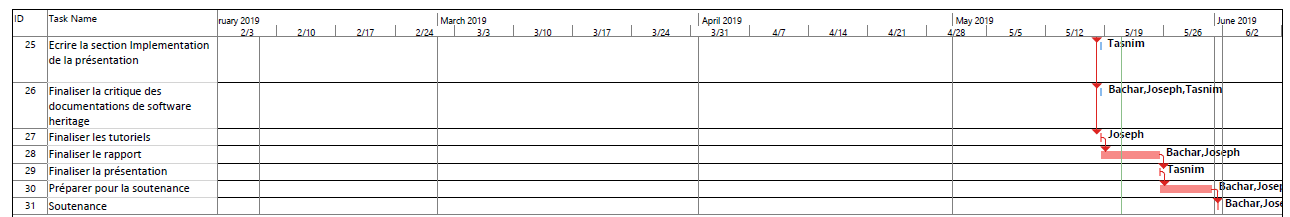
\includegraphics[scale=0.57]{images/planning_prev_p2.PNG}
\caption{Planning prévisionel}
\end{figure}

\section{Planning Final}
\begin{figure}[!ht]
\hspace*{-3.5cm}                
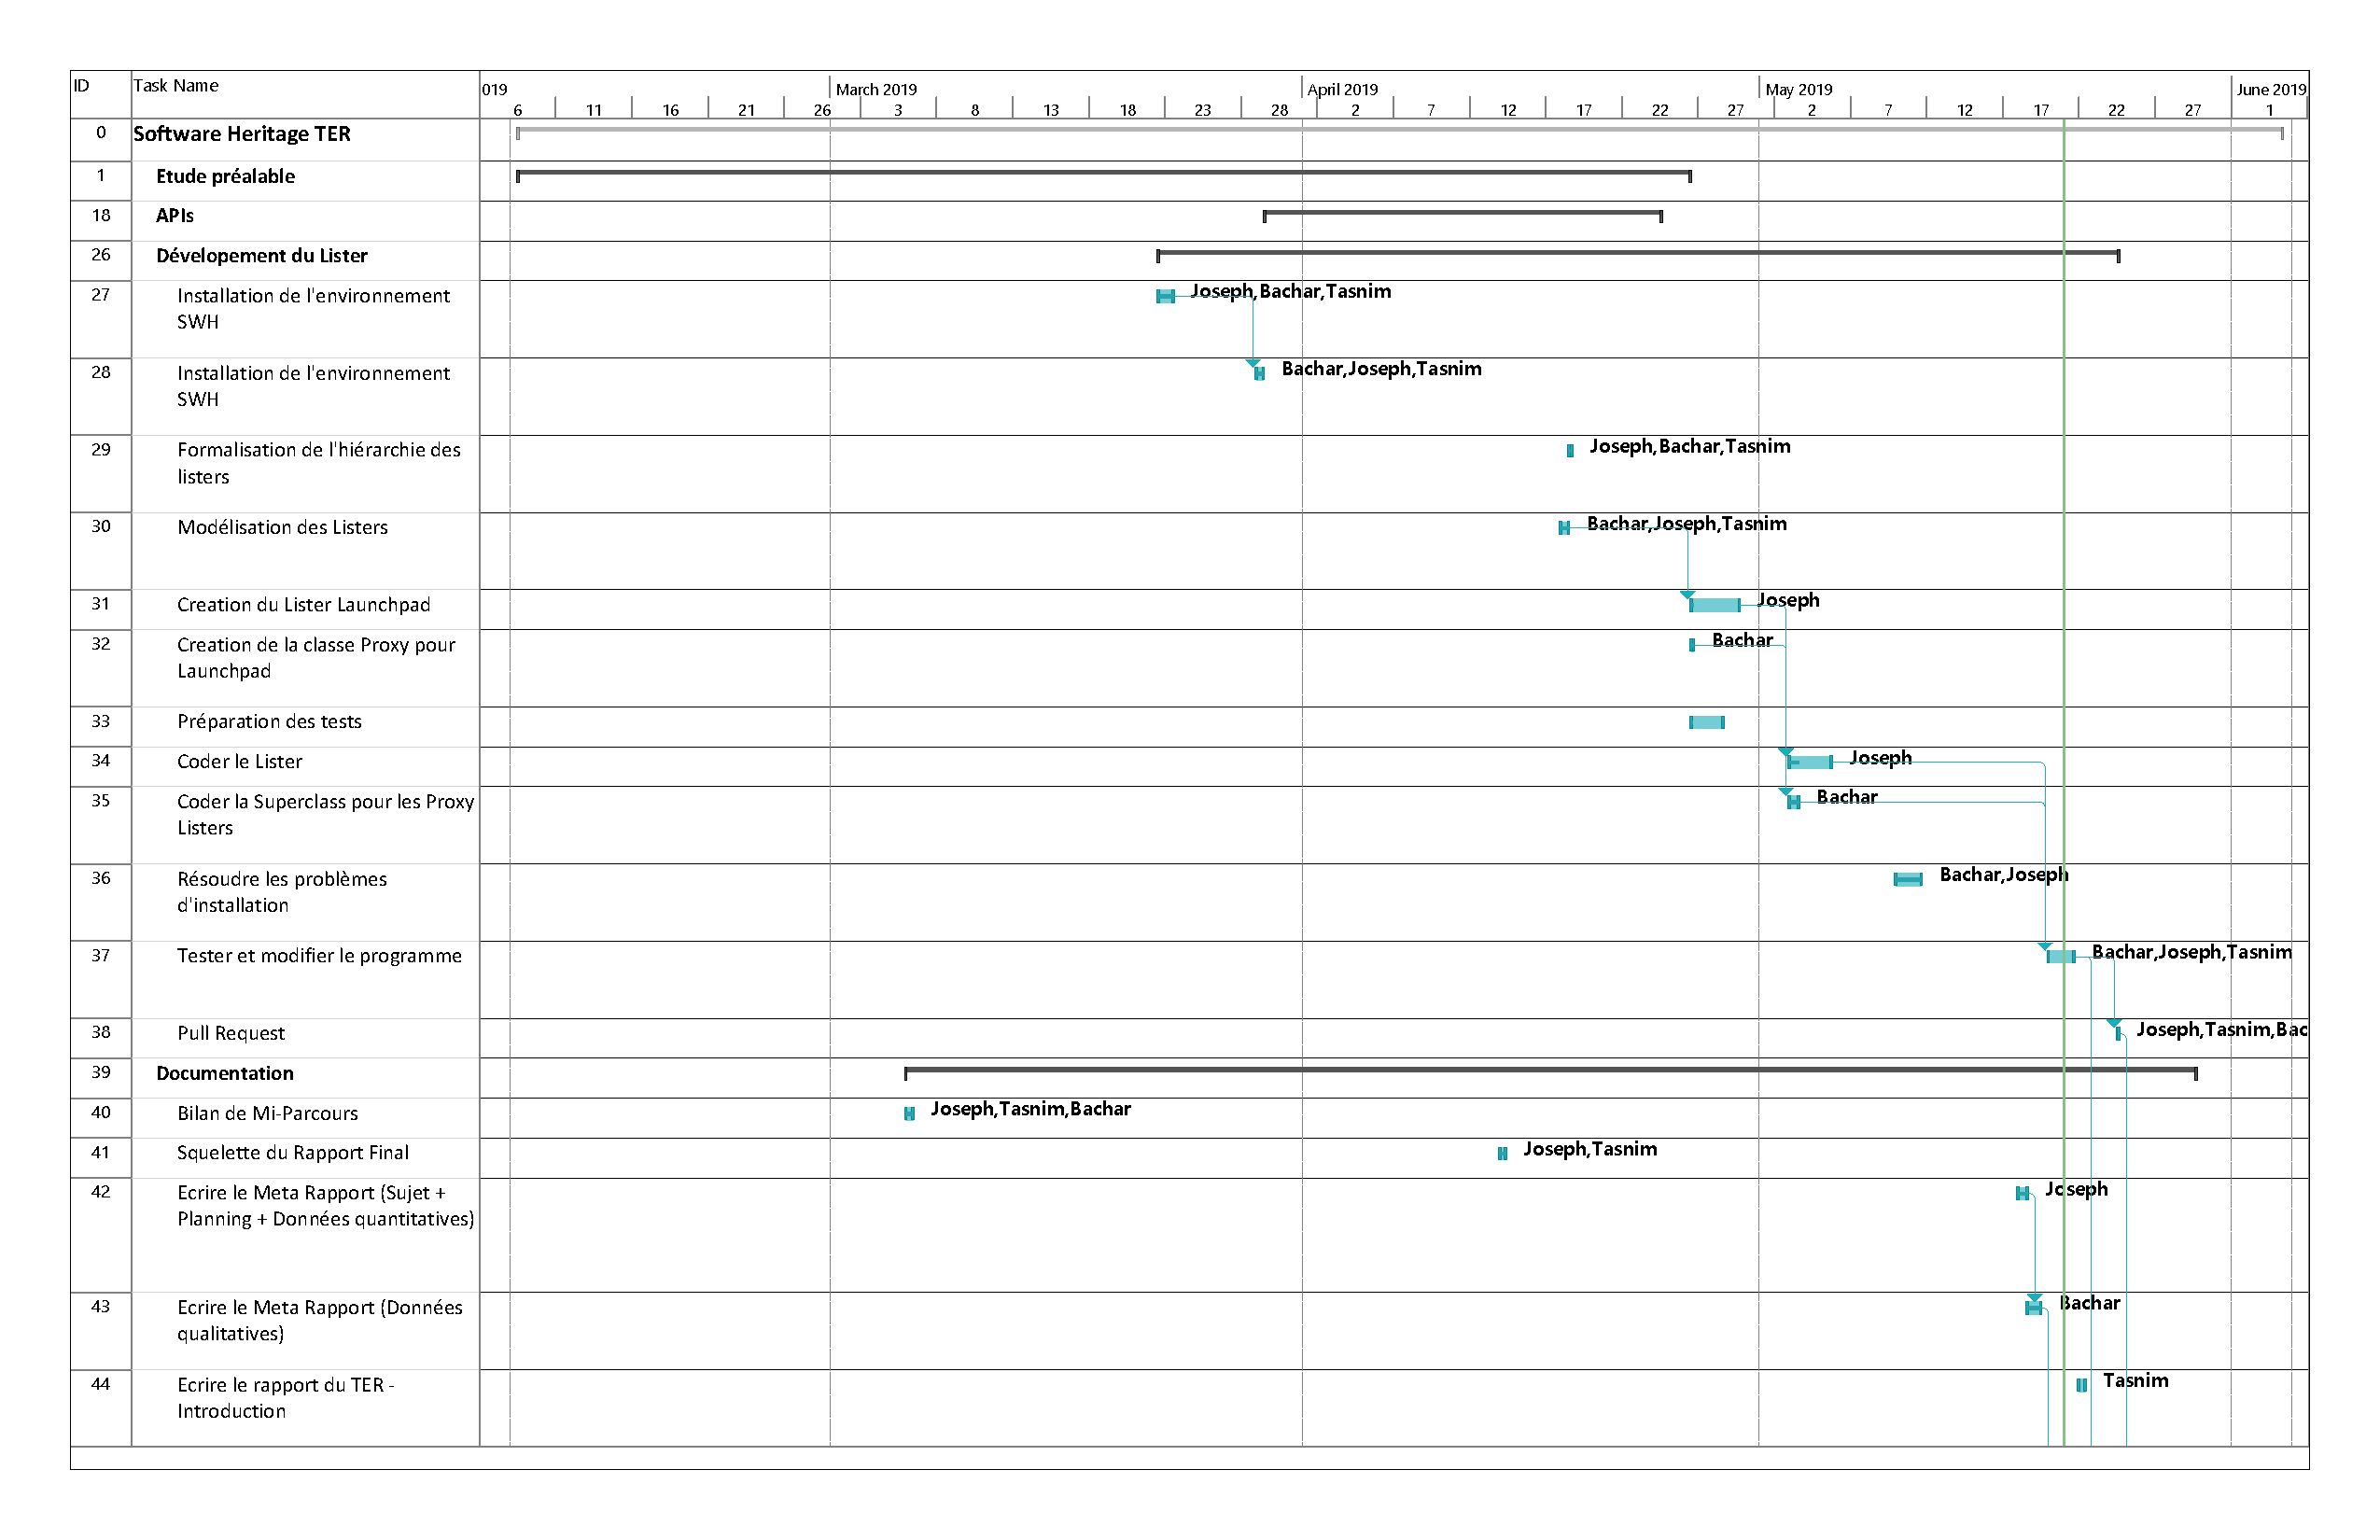
\includegraphics[scale=0.48]{planning_final_summary.pdf}
\end{figure}
%\includepdf[pages=2-,pagecommand={}]{planning_final_summary.pdf}
\begin{figure}[!ht]
\hspace*{-3.5cm}                
\includegraphics[scale=0.48,page=2]{planning_final_summary.pdf}
\caption{Planning final}
\end{figure}
\newpage
\section{Notes sur le planning final}
Aprés avoir déposer le planning prévisionnel, nous avons refait le planning et nous l'avons découpé en cinq parties pour mieux refléter la structure du projet:
\begin{itemize}
  \item \textbf{Étude préalable :} Cette section forme une grande partie du projet. Elle inclut toutes les tâches de lecture et recherche qui nous ont permis de se familiariser avec l'architecture et l'environnement de Software Heritage, ainsi que les differents Listers préexistants.
  \item \textbf{APIs :} Cette section regroupe les tâches qui concernent la recherche d'un dépot de code avec une API adaptée, qui va être éxploitée dans les tâches de développement.  
  \item \textbf{Développement du Lister :} Ce groupe contient les tâches liées au développement du Lister, donc les tâches de modélisation et conception, de coding, et de testing.
  \item \textbf{Documentation :} Pour organiser la création des rapports et de la présentation.
  \item \textbf{Soutenance :} Pour organiser les répétitions et la soutenance.
\end{itemize}

\section{Comparaison des plannings}
Bachar
\chapter{Données Quantitatives}
Ce chapitre ce concentre sur les details quantitatives concernant le TER. Le projet est disponible sur le lien Git suivant: \url{https://github.com/joe11093/Software-Heritage-TER}
\section{Commits}
Depuis la date de la création du Git repo, jusqu'au XX/XX/XXXX, nous avons effectué XX commits.

%graph de contributions Git
\begin{figure}[!ht]
\hspace*{-2.6cm}                
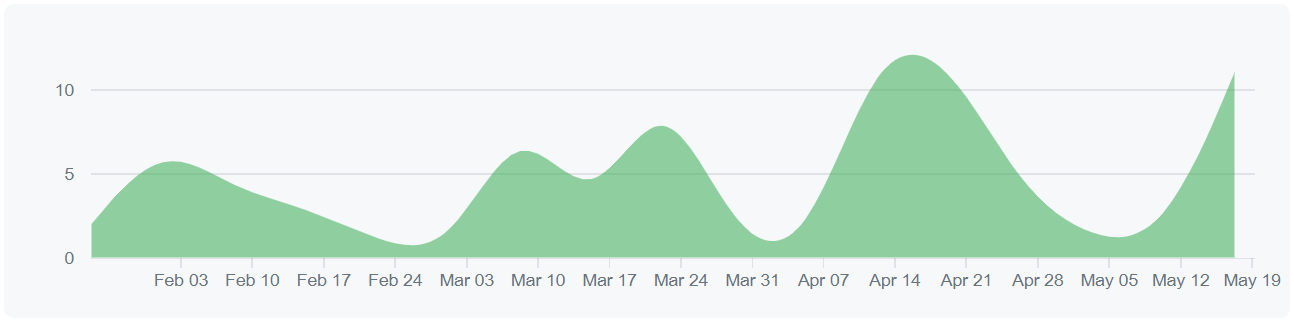
\includegraphics[scale=0.55]{images/contributor_graph_git.PNG}
\caption{Graph des commits}
\end{figure}

Nous observons qu'en premier temps, le nombre de commits est bas. Cela correspond à  la période de l'étude préalable qui consistait surtout de tâches de lecture. 
Les deux points bas suivants (aux alentour de fin Mars et début Mai) sont dû à la période de rattrapage et la période des révisions des examens finaux.
Les commits s'élèvent à la fin du TER parceque nous ajoutons au fur et à mesure le code sur lequel nous travaillons, ainsi que les rapports et leurs documents correspondants.

%graph des commits par jour de la semaine
%
\begin{figure}[!ht]
\hspace*{-4cm}                
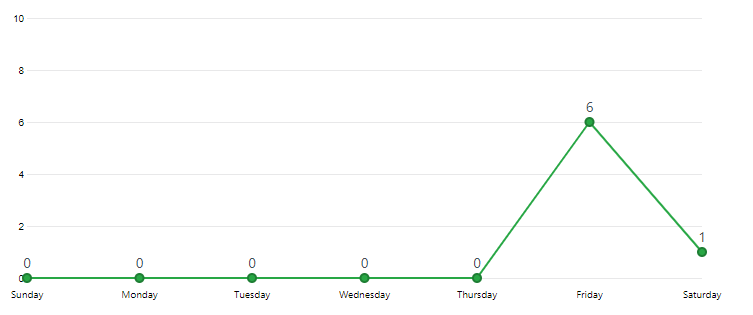
\includegraphics[scale=0.60]{images/contributor_week_feb3.PNG}
\hspace*{1.6cm}    
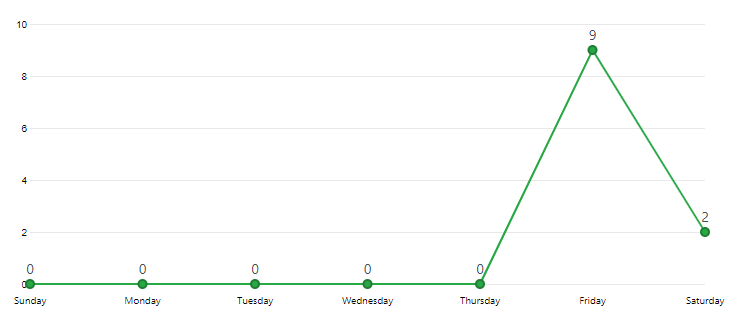
\includegraphics[scale=0.60]{images/contributor_week_march24.PNG}
\caption{Moyenne des commits par jours pour les semaines du 3 Février et du 24 Mars}
\end{figure}

Nous observons que les commits ont été souvent éffectué les Vendredis. En effet, nous avons decidé de travailler sur le TER les Vendredis, qui est la seule journée oú les trois membres du groupe n'ont pas de cours. Les commits de la dernière période du projet sont une éxception; cela est dû à l'arrêt des cours.  

\section{Classes}
\begin{itemize}
\item \textbf{LaunchpadProxy :} Cette classe éxploite l'API de Launchpad pour récupérer tous les projets Git disponibles publiquement.
\item \textbf{LaunchpadGitModel : } Elle définit le modèle d'un repository en Git hébergé sur Launchpad.
\item \textbf{LaunchpadGitLister : } La classe du Lister qui implemente toute les fonctions requises pour énumérer les origines hébergés sur Launchpad.
\item \textbf{ProxiedLister : } Classe abstraite qui pourra être implementée dans un autre Lister qui a les éxigences que Launchpad.
\item \textbf{WebApiProxy : } Une interface qui contient les déclarations des fonctions requise dans une classe Proxy utilisée par un Lister.
\item \textbf{LaunchpadListerTester :} Une classe utilisée dans les tests
\end{itemize}

\section{Temps de Travail}
En ce qui concerne le temps de travail, nous estimons:
\begin{itemize}
\item Approximativement 110 heures sur l'étude préalable du projet.
\item Approximativement 60 heures pour la recherche et les tests des APIs.
\item Approximativement 110 heures pour le developpement du code
\item Approximativement 20 heures pour la documentation et les rapports.
\item Approximativement 
\end{itemize}

Nous estimons encore autour de 30 heures de travail, qui portera surtout sur l'écriture du rapport du TER ainsi que la présentation.
\chapter{Conclusion}




\end{document}